\chapter{Implementation}
\label{chap:implementation}
This has the description of how you actually went about implementing the project.  This should be focused on the interesting challenges and how those related to the project.

\todo{add more here. if you are reading this you can see that I am using todo as a way to indicate where the updates should be}


For code listing we have decided to use the lstlisting package. There are several ways to use the package.  The basic use is a code listing inline see Listing~\ref{lst:HelloWorldC++} for a \CPP example and Listing~\ref{lst:Python} for a Python example. The listings package does the work of colourizing cose so that you can easily include formatted code.   For more documentation on listings on wikibooks \footnote{\url{https://en.wikibooks.org/wiki/LaTeX/Source_Code_Listings}}

%these are the default setup for code blocks 
\lstset{frameround=tttt}
\lstset{frame=single}
\lstset{xleftmargin=.05\textwidth, xrightmargin=.05\textwidth}


\begin{lstlisting}[language=C++, caption= {Hello World C++ The code listing for Hello World in C++, with colour syntax highlighting.}, label={lst:HelloWorldC++}]
    #include<stdio.h>
    #include<iostream>
    // A comment
    int main(void)
    {
        printf("Hello World\n");
        return 0;
    }
\end{lstlisting}

\lstset{language=Python}
\begin{lstlisting}[caption = {The code listing for a Python increment a matrix example}, label={lst:Python}]
    import numpy as np
    x = 1
    a = np.array([[1.0, 2.0], [3.0, 4.0]])
    if x == 1:
        # indented four spaces
        print("x is 1.")
        print("Hello World")
        print(a)
\end{lstlisting}


We have many students using Go as a programming language.  It is too new to have a definition in \LaTeX so we will create one temporarily until the listing package adds it. You can see the result in Listing~\ref{lst:HelloWorldGo}

\lstdefinelanguage{go}
    {   morekeywords={var, for, int, string , float, struct, func, package, import},
        sensitive=false,
        morecomment=[l]{//},
        morecomment=[s]{/*}{*/},
        morestring=[b]",
        basicstyle=\ttfamily,
        keywordstyle=\color{red}\ttfamily,
        stringstyle=\color{darkgreen}\ttfamily,
        commentstyle=\color{blue}\ttfamily,
    }

\begin{lstlisting}[language=go, caption={Go code for hello world}, label={lst:HelloWorldGo}]
    package main

    import "fmt"
    func main() {
        fmt.Println("hello world")
    }
    
\end{lstlisting}




We also think it is useful to be able to link content from the files directly.  In the tables example we used csvsimple.  Here we can use the feature \lstinline{\lstinputlisting} with options for first line and last line see Listing~\ref{lst:HelloWorldC++file}.

%nice way to link to a file directily
\lstinputlisting[language=C++, firstline=2, lastline=12,caption={Hello World in C++ from a file}, label={lst:HelloWorldC++file}]{inc/helloworld.cpp}

There is also an interesting challenge related to visual programming languages.  As these become more common, particularly Blueprints in Unreal Engine, we need to have a listing option for visual code.  This is a bit of a workaround as listings are normally code but we use an escape sequence in the listing to include the graphic see Listing~\ref{lst:blue1}.

%create escape sequence
\lstset{
    escapeinside={(*@}{@*)},          % if you want to add LaTeX within your code
}

% define blueprint as a programming language with no real text keywords or syntax and no margins
\lstdefinelanguage{blueprint}{
    morekeywords={visual},
    sensitive=false,
    frame=none, 
    xleftmargin=0pt, 
    xrightmargin=0pt
}

\begin{lstlisting}[language=blueprint, caption={Blueprint from Unreal Engine}, label={lst:blue1}]
    (*@ 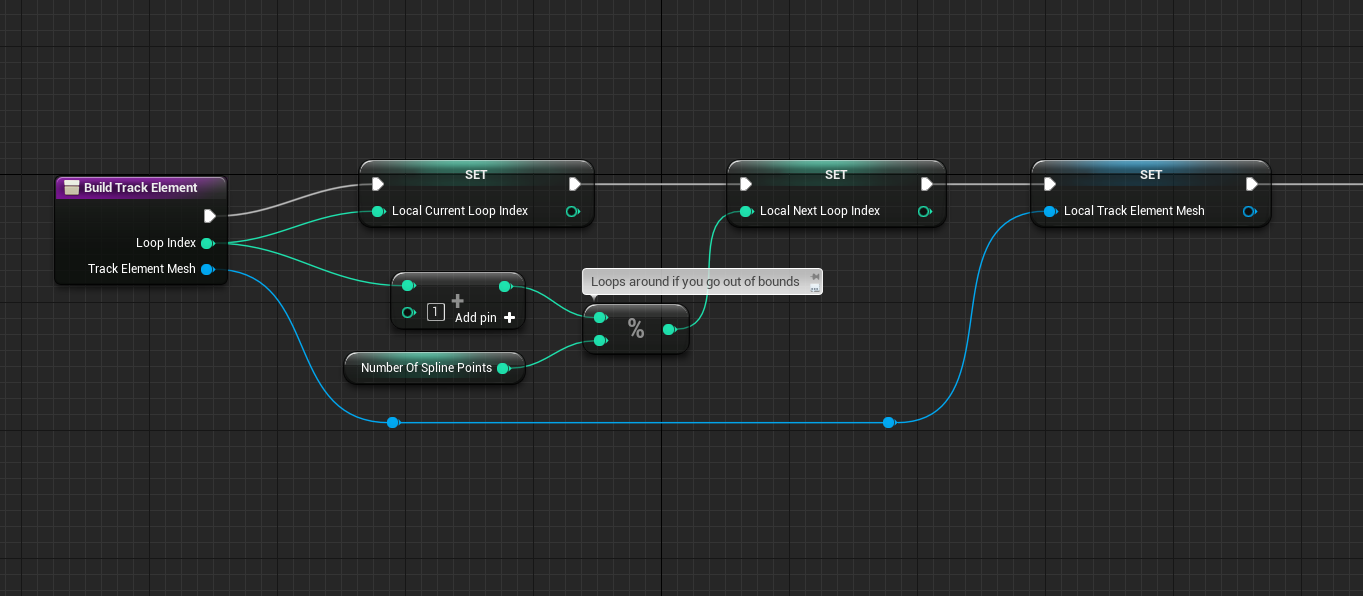
\includegraphics[width=.90\textwidth]{images/blueprint} @*)
\end{lstlisting}


Students have also suggested the minted package for pretty code listings.  We will consider this in future updates to the coding style at NTNU.



